%!TEX root = these.tex

\chapter{Communication en streaming et en temps réel avec les codes optiques}

Ce chapitre présente une version reformatée et traduite d'un article publié en 2016 dans IEEE Access, v.4, p.284-298 par K. Xie, S. Gaboury et S. Hallé.

%% -----------------------
%% Section: intro
%% -----------------------
\section{Introduction}\label{sec:qr:intro} %% {{{

La communication sans fil est une technologie qui permet à deux ou plusieurs pairs de communiquer sans câbles électriques ou conducteurs \citep{tse2005fundamentals}. Alors que la majorité des technologies de communication sans fil utilise les ondes radio comme leurs milieux de transmission, quelques autres utilisent la lumière, en particulier dans les situations où la technologie radio est difficile à fonctionner. La communication optique en elle-même remonte à l'utilisation de drapeaux, les signaux de fumée et les lampes signalétiques pour communiquer de l'information entre deux points avec l'utilisation d'un code spécifique \citep{burns2004}.

Récemment, une forme simple de communication optique, appelée \emph{Quick Response Code} (code QR) \citep{qrcode-about}, a émergé comme un raffinement de la technologie existante de code-barres unidimensionnels. En raison de leur exactitude et leur grande capacité, les codes QR ont été utilisés dans de nombreux domaines; les applications du traitement de tels codes ont également été portés à une variété de dispositifs, y compris les ordinateurs de bureau, les smartphones, et même les télévisions.

Cependant, jusqu'à présent les codes QR ont été utilisés pour la transmission de données statiques. En général, un code est imprimé sur un milieu physique, tel qu'une feuille de papier, et il est lu par un appareil optique (généralement une caméra) pour le décodage à un moment ultérieur. Dans ce chapitre, nous explorons l'idée de l'expansion de codes QR et les transformons en un canal dynamique de communication unidirectionnelle. Dans un tel canal, un flux de données est transmis par une \emph{séquence de codes}; généralement, ces codes sont continuellement générés et affichés sur un appareil, et simultanément capturés et décodés par un autre, ce qui est similaire aux autres types de technologies de communication.

Après avoir brièvement décrit dans la Section~\ref{sec:qr:reading} les bases de codes QR et d'autres technologies de communication sans fil, nous nous concentrons dans la Section~\ref{sec:qr:qrcode} sur le principe de communication de codes QR bruts. Particulièrement, nous essayons de trouver les limites intrinsèques d'un tel canal de communication, par l'analyse de l'influence de divers facteurs, tels que la densité de code, le nombre de codes affichés par seconde, etc. Les résultats d'un benchmark qui couvrent plus de cent combinaisons différentes de paramètres permettent d'extraire les conditions optimales qui minimisent le taux d'erreur dans le décodage des images, tout en maximisant la quantité de données qui peuvent être transmises par unité de temps.

Ces premiers résultats indiquent que les flux de codes QR peuvent en effet être utilisés comme un canal simple et unidirectionnel, mais que la communication sans erreur et la bande passante élevée sont plus ou moins impossibles. Par conséquent, en tant qu'un deuxième temps, nous concevons un protocole qui est approprié pour la nature spécifique de communication de codes QR. Ce protocole, appelé BufferTannen, est décrit dans la section~\ref{sec:qr:protocol}. Il est capable d'encapsuler les données brutes, de fournir diverses capacités de signalisation, de pouvoir représenter les données semi-structurées (telles que JSON) sous une forme binaire compacte, et prend en charge le cadrage/décadrage et le streaming de données.

Une seconde expérience révèle la robustesse de ce schéma de transmission: en utilisant notre protocole spécialement conçu, le canal de communication créé par une personne qui pointe un smartphone à bout de bras vers un écran avec les codes QR des codes QR vacillants, produit une bande passante suffisante pour transmettre l'audio à usage vocal en temps réel. La Section~\ref{sec:qr:experiments} présente l'environnement et les résultats des expériences de cette deuxième étape. Nous montrons aussi comment un morceau de données, coupé en plusieurs codes avec l'utilisation de BufferTannen, peut être reconstruit automatiquement par un utilisateur qui passe sa caméra sur une feuille de ces codes imprimés dans aucun ordre particulier.

Ce travail a été motivé par une application pratique dans le domaine de la vérification de l'exécution. Dans les recherches antérieures, nous avons proposé et officieusement expérimenté l'utilisation de codes optiques comme une forme de communication à couplage lâche entre un système logiciel et un moniteur externe qui reçoit les événements produits par ce système-là \citep{DBLP_conf/rv/LavoieLVGH14}. Dans ce contexte, la communication par les milieux optiques assure un isolement complet entre le système et son moniteur.

Bien que l'utilisation de séquences de codes QR a été officieusement suggéré dans le passé, au mieux de notre connaissance, notre recherche est la première enquête systématique du potentiel de codes QR pour envoyer les flux de données en temps réel.

La solution que nous proposons fournit une méthode pour distribuer les données en streaming sans dispositifs dédiés de communication. Les appareils requis sont seulement une caméra commune (comme une webcam ou la caméra dans un téléphone portable) et une petite surface plane pour afficher les codes QR séquentiels --- par exemple, un écran d'ordinateur, une télévision ou un smartphone, ou même une feuille de papier.
%% }}} --- Section

%% -----------------------
%% Section: comment on lit les codes QR
%% -----------------------
\section{Communications sans fil}\label{sec:qr:reading} %% {{{

Cette section rappelle quelques technologies communes de communication sans fil. Malgré leur popularité et leur performance, chacune a ses propres limites et ses scénarios d'application.

\subsection{Ondes Radio}

Le premier milieu évident de communication sans fil est grâce à l'utilisation d'ondes radio, dont le meilleur exemple est WiFi \citep{Comer:2008:CNI:1816918}, utilisé pour la mise en réseau sans fil de la zone locale. Ses variantes sont basées sur la famille de standards IEEE 802.11, et prennent en charge la mise en réseau centralisée (routage) et décentralisée (\textit{ad hoc}). Le Tableau \ref{tab:qr:wifi-protocol} montre les standards populaires de 802.11 et une partie de leurs spécifications.

\begin{table}[ht]
\begin{center}
\begin{tabular}{|c|c|c|c|}
\hline
Protocole &	Fréquence & Débit maximal de données physiques	&	Portée intérieure \\
\hline
802.11a &	5 GHz &	54 Mbps &	35 m \\
\hline
802.11b &	2.4 GHz &	11 Mbps &	35 m\\
\hline
802.11g &	2.4 GHz &	54 Mbps &	38 m\\
\hline
802.11n &	2.4/5 GHz &	150 Mbps &	70 m\\
\hline
802.11ac &	5 GHz &	866.7 Mbps & 35 m\\
\hline
\end{tabular}
\caption{Résumé des protocoles WiFi \citep{theng2008ubiquitous,perahia2013next}}
\label{tab:qr:wifi-protocol}
\end{center}
\end{table}

Un deuxième concurrent dans cette famille est Bluetooth \citep{Comer:2008:CNI:1816918}, qui est utilisé à courte portée et généralement comme communication point à point entre les appareils. Sa portée varie d'environ 1 à 100 mètres en fonction de la classe d'énergie. Le Tableau \ref{tab:qr:bluetooth} montre différentes versions de Bluetooth et leurs débits de données spécifiques.

\begin{table}[ht]
\begin{center}
\begin{tabular}{|l|r|c|}
\hline
Version &	Débit de données	&	Portée \\
\hline
Version 1.2 &	1 Mbps &	\multirow{4}{*}{\pbox{20\textwidth}{Classe 1: 100 m; \\ Classe 2: 10 m; \\ Classe 3: 1 m}}\\
\cline{1-2}
Version 2.0 + EDR &	3 Mbps & \\
\cline{1-2}
Version 3.0 + HS &	24 Mbps & \\
\cline{1-2}
Version 4.0 &	24 Mbps & \\
\hline
\end{tabular}
\caption{Spécifications de Bluetooth \citep{gupta2013inside}}
\label{tab:qr:bluetooth}
\end{center}
\end{table}

Enfin, ZigBee \citep {farahani2011zigbee}, basé sur le standard IEEE 802.15.4, vise à mettre en œuvre une communication sans fil à courte portée avec une faible énergie et une batterie de longue durée. Le Tableau \ref{tab:qr:zigbee} montre ses performances dans différentes bandes de fréquences.

\begin{table}[ht]
\begin{center}
\begin{tabular}{|l|r|c|}
\hline
Bande de fréquence & Débit de données	&	Portée \\
\hline
868--870 MHz &	20 kbps &	\multirow{3}{*}{\pbox{5 cm}{10--100 m, en fonction de la puissance de sortie et de l'environnement}}\\
\cline{1-2}
902--928 MHz &	40 kbps & \\
\cline{1-2}
2.4--2.4835 GHz  &	250 kbps & \\
\hline
\end{tabular}
\caption{Spécifications de ZigBee \citep{lee2007comparative}}
\label{tab:qr:zigbee}
\end{center}
\end{table}

Tous ces protocoles partagent un point commun: avant d'autoriser toute forme de communication entre deux extrémités, une certaine forme de \emph{découverte} ou \emph{configuration} de dispositifs est nécessaire. Ce processus est généralement achevé à travers l'établissement d'une \emph{connexion} avec états à long terme entre les extrémités.

\subsection{IrDA}

Dans une autre famille, on trouve des technologies utilisant des ondes infrarouges au lieu du signal radio \citep{sarkar2007ad}. Outre les longueurs d'onde différentes, ces technologies assouplissent généralement les exigences de l'établissement d'une connexion, et permettent une communication plus ``on-the-fly'' entre deux appareils. En règle générale, une extrémité d'une liaison infrarouge attend les données entrantes, tandis que périodiquement, un autre appareil pointe au récepteur et émet les rayons infrarouges transformés à partir de petits morceaux de données sans nécessité de préavis.

Une importance particulière est le standard IrDA (Infrared Data Association); ses émetteurs envoient des impulsions infrarouges avec un angle de cône et une irradiance modérée alors que ses récepteurs peuvent être à moins d'un mètre ou plusieurs mètres de ceux-là, en fonction de l'énergie des émetteurs et de la position dans le cône. La communication IrDA est semi-duplex et fournit CRC de base. Le Tableau \ref{tab:qr:irda-rate} montre plusieurs schémas IrDA et leurs débits de données dans la portée spécifique.

\begin{table}[ht]
\begin{center}
\begin{tabular}{|l|c|c|}
\hline
Schéma & Débit de données & Portée \\
\hline
SIR &	2.4--115.2 kbps &	\multirow{4}{*}{\pbox{3 cm}{jusqu'à un mètre}} \\
\cline{1-2}
MIR &	0.576--1.152 Mbps & \\ 
\cline{1-2}
FIR &	4 Mbps & \\
\cline{1-2}
GigaIR &	512 Mbps--1 Gbps & \\
\hline
\end{tabular}
\caption{Débits de données de schémas de couche physique de IrDA \citep{millar1998irda}}
\label{tab:qr:irda-rate}
\end{center}
\end{table}

\subsection{Visible Light Communication}

Comme l'indique son nom, Visible Light Communication (VLC) \citep{komine2004fundamental} utilise des longueurs d'onde dans la gamme visible (400-700 nm) pour communiquer les données entre les pairs --- ceci est généralement réalisé par allumer et fermer rapidement une source de lumière, ce qui permet une forme de codage des données comme les codes Morse. Un récepteur (par exemple une cellule photo-électrique) pointé par la source de lumière détecte ce vacillement et le convertit en données numériques. Avec les lampes fluorescentes comme la source lumineuse, le débit de données peut atteindre 10 kbps, tandis qu'avec la technologie LED, le débit de données peut être aussi élevé que 500 Mbps. La gamme dépend surtout des spécifications différentes, mais comme la lumière ne peut pas traverser les murs et peut également être affectée par le mauvais temps ou d'autres sources de lumière, sa portée et sa fiabilité sont limitées~\citep{arnon2015visible}.

Ce mode de communication est intrinsèquement unidirectionnel, car on ne peut pas répondre à la source de lumière, reconnaître la réception de l'information, ou demander d'une retransmission en cas de la perte de données. Par conséquent, cette technologie est aussi celle qui nécessite le moins de couplage entre un émetteur et un récepteur; selon tous les moyens pratiques, l'émetteur n'a pas connaissance de la présence d'un récepteur, qui, de son côté, peut choisir de commencer à recevoir à tout moment. Nous verrons plus loin que cette caractéristique est également partagée avec le canal de communication de codes QR que nous essayons de concevoir.

%% }}} --- Section

%% -----------------------
%% Section: le protocole
%% -----------------------
\section{Flux de codes QR}\label{sec:qr:qrcode} %% {{{

Dans le court sondage précédent de technologies de communication sans fil sont mentionnés les codes optiques, qui sont aussi un moyen de transport de données sans nécessité d'un milieu physique. Dans cette section, nous passons en revue le concept de codes QR, et discutons de l'idée de produire les flux de données par les séquences de tels codes.

\subsection{Aperçu de codes QR}

Un code QR (officiellement appelé ``Quick Response Code'') \citep{qrcode-about} est un code-barre à deux dimensions qui stocke des données, comme le montre la figure \ref{fig:qr:helloqr}. En comparaison avec le code-barre bien connu UPC, qui est linéaire (i.e.\ unidimensionnel), un code QR peut stocker plus d'informations dans une impression plus petite.\footnote{\url{http://www.qrcode.com/en/}} Le standard du code QR stipule que ces codes peuvent avoir une capacité aussi élevée que 7089 caractères numériques ou 2953 caractères à 8 bits, et qu'un code est représenté dans un tableau carré d'un maximum de 177 $\times$ 177 ``pixels'', appelé \emph{modules} \citep{iso18004}.

\begin{figure}
\centering
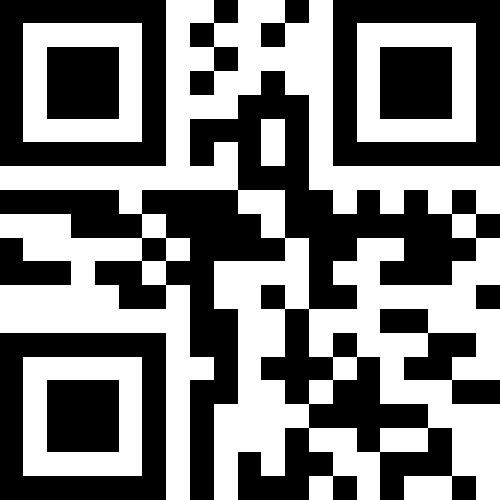
\includegraphics[width=1in]{helloqr.png}
\caption{Un code QR avec le texte ``Hello world!''}
\label{fig:qr:helloqr}
\end{figure}

\begin{table}[t]
\begin{center}
\begin{tabular}{|c|c|c|c|c|c|}
\hline
Niveau de & Bits de & Caractère  & Caractère  & Caractère & Kanji \\
correction d'erreur & données & numérique & alphanumérique & binaire & \\
\hline
L &	23,648 & 7,089 & 4,296 & 2,953 & 1,817\\
\hline
M & 18,672 & 5,596 & 3,391 & 2,331 & 1,435\\
\hline
Q & 13,328 & 3,993 & 2,420 & 1,663 & 1,024\\
\hline
H & 10,208 & 3,057 & 1,852 & 1,273 & 784\\
\hline
\end{tabular}
\caption[Capacités]{Capacités maximales de stockage de codes de la version 40}
\label{tab:qr:qrcode-capacity}
\end{center}
\end{table}

La capacité d'un code QR dépend principalement de son type de données, de sa version et de son niveau de correction d'erreur. Le type de données peut être \emph {uniquement numérique}, \emph{alphanumérique}, \emph{binaire}, ou \emph{Kanji}. La version de 1 à 40, détermine les dimensions d'un code, qui varient de 21 $\times$ 21 à 177 $\times$ 177 modules. Les codes QR utilisent une forme de codage de correction d'erreur qui agit à quatre niveaux: \emph{Low} (L), \emph{Medium} (M), \emph{Quartile} (Q), et \emph{High} (H), comme il est indiqué dans le Tableau~\ref{tab:qr:qrcode-capacity}. Évidemment, comme le niveau augmente, plus de redondance est introduite dans le contenu du code, ce qui diminue sa capacité de stockage; cependant, plus de données peuvent être restaurées si le code est sale ou endommagé. Avec les formes de détection de position incluses dans le symbole, un code QR peut être décodé en 360 degrés.

Avant de générer un code QR à partir d'un morceau de données, un générateur de code doit analyser les données d'entrée pour décider du mode et de la version les plus efficaces. Dans le codage de données, les caractères sont convertis en un flux de bits, et dans ce progrès, certains \emph{indicateurs de mode} et \emph{terminateurs} sont insérés pour les changements de mode. Le flux de bits est ensuite divisé en mots de code à 8-bits, et les caractères de remplissage sont nécessaires pour combler le nombre de mots de code de la version choisie. La séquence de mots de code générée est divisée en blocs selon le niveau de correction d'erreur spécifique et un mot de code de correction d'erreur est généré pour chaque bloc. Ensuite, les mots de code de chaque bloc sont entrelacés et quelques bits restants sont ajoutés selon le besoin.

Dans l'étape suivante, le générateur met les modules de mots de code dans une matrice en noir et blanc avec la forme de recherche, les séparateurs, la forme de synchronisation et les formes d'alignement; il applique les formes de masquage, évalue et sélectionne ensuite la forme appropriée. Enfin, il génère le \emph{format} et \emph{l'information de version} et complète le code QR \citep{iso18004}.

Les étapes de décodage ne sont que tout simplement l'inverse de la procédure de codage. Dans un premier temps, le code QR doit être situé et les modules noirs et blancs sont reconnus comme 0s et 1s qui forment un tableau binaire. De ce tableau binaire, le décodeur reçoit l'information du format et de la version. Avec ces informations, il peut commencer à lire les caractères et les mots de code de correction d'erreurs, puis tente de détecter et de corriger les erreurs avec les mots de code de correction d'erreurs selon le niveau de correction d'erreur approprié. Dans l'étape suivante, les mots de code de données sont divisés selon le \emph{indicateurs de mode} et les \emph{indicateurs de nombre de caractères}, et les caractères de données sont finalement décodés et sortis.

\subsection{Le cas de communication de codes QR}

Le processus précité s'applique au codage et au décodage d'un code unique contenant des données statiques. Nous enquêtons maintenant sur l'idée d'utiliser les codes QR en tant qu'un canal de communication, où les données en temps réel seraient transformées en situation réelle comme une \emph{séquence} de codes QR, qui pourraient ensuite être optiquement capturées par un dispositif, et reconverties en flux de données d'origine à l'extrémité de réception.

L'utilisation de communication de codes QR présente plusieurs avantages dans une poignée de scénarios. Par exemple, la Marine américaine a enquêté sur l'utilisation de codes QR comme un ``sémaphore numérique''. La technologie proposée se concentre sur la détection de codes à basse résolution à partir de très longues distances, et souligne l'intérêt et les cas possibles d'utilisation de cette technologie dans un contexte militaire:

\begin{quote}
``Arguably the most significant advantage of QR code LOS [line of sight] communications is the fact that they can be conducted without emitting energy in the RF spectrum. In an emissions controlled (EMCON) environment, this will provide a critical ability to communicate between ships without increasing the possibility of position detection.'' \citep[p.\ 46]{richter-msc}
\end{quote}

Cependant, dans l'ouvrage cité, les codes sont considérés comme \emph{statiques}, c'est-à-dire qu'ils ne changent pas au fil du temps pour former un flux de données, et agissent plus ou moins comme un substitut de drapeaux ou de signes. Néanmoins, l'absence de toute émission d'ondes radio dans la communication de codes QR s'avère un avantage attrayant dans certains scénarios.

Nous avons également vu dans la section précédente comment toutes les autres technologies, telles que Bluetooth ou IrDA, nécessitent un matériel spécialisé. En revanche, la communication de codes QR peut être réalisée à travers les codes imprimés sur une surface dure, ou par un dispositif capable d'afficher des images à une résolution suffisante: les écrans de télévision, les écrans d'ordinateur, les tablettes et les téléphones cellulaires. De même, la réception peut être faite par un appareil équipé d'une caméra commerciale normale. Cela peut convertir les appareils équipés de ce matériel courant en dispositifs de communication, même s'ils ne sont pas conçus à cet effet en premier lieu. On peut même imaginer les situations d'urgence dans lesquelles tous les moyens numériques de communication entre deux points ne fonctionnent pas. Si la ligne de vision peut être établie et un affichage et une caméra sont disponibles, l'utilisation de codes QR permet néanmoins de transmettre les données numériques --- sans doute beaucoup plus rapidement que le manuel écriture ou transcription.

Enfin, nous avons mentionné au début comment l'utilisation d'un canal de communication optique et strictement unidirectionnelle peut également être souhaitable, même dans les situations où la communication radio ou câble est disponible. Par exemple, dans le contexte de la vérification de l'exécution, l'exécution d'un système est actuellement observée par un processus externe appelé \emph{moniteur}. Pour empêcher le moniteur d'interférer avec l'exécution du système, il est souvent placé sur une machine séparée, avec un canal de communication qui transporte les événements du premier au second. Cependant, dans les protocoles traditionnels tels que TCP, la nature bidirectionnelle d'une connexion présente un risque trop élevé d'attaques contre le programme de monitoring. En outre, certaines configurations de logiciels sont nécessaires pour brancher le moniteur au programme: les adresses IP, les noms de tube, les ports, etc., ce qui représente trop de couplage dans de nombreux scénarios. Nous avons discuté dans le travail précédent \citep{DBLP_conf/rv/LavoieLVGH14} comment l'utilisation d'un canal de communication optique peut atténuer ces problèmes en fournissant un plus grand isolement entre le système et son moniteur.

\subsection{Estimation de la bande passante et du taux d'erreur}

Cependant, la transmission unidirectionnelle introduit la possibilité de perte d'images pendant le procédure, en raison de la limitation des dispositifs physiques ou la vulnérabilité du logiciel. De plus, c'est impossible que l'émetteur puisse être conscient d'images manquantes à l'extrémité de réception et les renvoyer. Par conséquent, nous avons besoin d'analyser profondément cette approche pour estimer le \emph{taux de reconnaissance} et la \emph{bande passante de transmission} d'un tel canal de communication.

La transmission de codes utilise plusieurs paramètres: la taille de données de chaque image, le nombre d'images générées par seconde (fps) et le niveau de correction d'erreur. Tous les trois peuvent avoir un effet important de la génération de codes QR et de la bande passante résultante. Une plus grande taille de données mène à une plus haute version de symbole de codes QR et plus de modules de symboles, et avec la même taille d'image, un niveau plus élevé de correction exige plus de modules de symboles qu'un niveau moins élevé.

Comme l'émetteur ne peut pas détecter le fait que des codes soient manqués ou non par le récepteur, ce canal de communication unidirectionnel est en fait un canal avec perte, dont la bande passante actuelle peut être calculée avec le taux mesuré de reconnaissance d'images. Cela représente le nombre de bits qui sont reçus correctement.

\begin{equation*}
  bande\_passante = \mathit{fps} \times \mathit{bits\_de\_image} \times \mathit{taux\_de\_reconnaissance}
\end{equation*}

Si le récepteur craint que les images ne sont pas tout reçues, la seule façon est de s'assurer que l'émetteur envoie toutes les images plusieurs fois jusqu'à ce que le récepteur reçoit toutes les images; alors la bande passante réelle est la suivante:

\begin{equation*}
  bande\_passante = \mathit{fps} \times \mathit{bits\_de\_image} \div \mathit{nombre\_de\_fois\_de\_envoi}
\end{equation*}

Le taux de reconnaissance est normalement déterminé par la capacité de la caméra et de l'écran, la précision de l'algorithme de reconnaissance et la complexité de codes (c.-à-d. le nombre des modules affichés). Cependant, dans la capacité de la caméra et de l'écran, si nous pouvons envoyer la même image plus d'une fois, et entre-temps la valeur de \emph{fps} n'a pas à changer, le taux pratique de reconnaissance peut être amélioré.

\begin{equation*}
\mathit{taux\_pratique\_de\_reconnaissance} = 1 - (1 - \mathit{taux\_de\_reconnaissance})^{nombre\_de\_fois}
\end{equation*}


%% }}} --- Section

%% -----------------------
%% Section: expériences
%% -----------------------
\section{Expériences}\label{sec:qr:experiments} %% {{{

Dans cette section, nous décrivons les expériences où nous mesurons la précision de reconnaissance de séquences de codes QR dans diverses conditions. Le but de ces expériences est triple:

\begin{enumerate}
\item évaluer si les données peuvent être transmises avec succès à travers la reconnaissance de séquences de codes optiques;
\item trouver les paramètres qui maximisent la vitesse de décodage et la bande passante des données transmises;
\item à partir de ces résultats, déterminer les caractéristiques d'un canal typique de communication de flux de codes QR.
\end{enumerate}

\subsection{Préparation des expériences}

Notre installation expérimentale implique la production et l'affichage de séquences de codes QR à une extrémité, et la capture et le décodage de ces séquences à l'autre extrémité. Dans notre environnement expérimental, nous avons utilisé un écran LED de 19 pouces de Samsung comme émetteur et une webcam Logitech à haute définition comme récepteur. La caméra était mise à une distance fixe de 50 cm de l'écran. La résolution de l'écran est de 1280 $\times$ 1024 pixels.

La caméra était mise sur une surface stable, avec la zone de code optique correctement mise au point et couvrant tout le champ de vision. L'ordinateur utilisé dans les expériences est un ordinateur portable avec le processeur Intel Core i7-3632QM et 16 Go de mémoire. La Figure \ref{fig:qr:setup} montre l'installation utilisée dans les expériences.

\begin{figure}
\centering
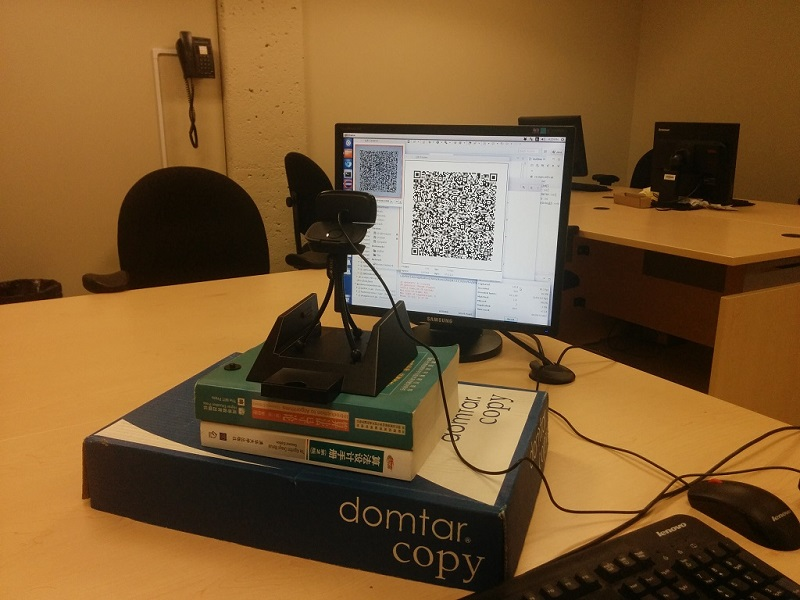
\includegraphics[width=\linewidth]{expsetup.jpg}
\caption{Installation expérimental pour lire les codes QR.}
\label{fig:qr:setup}
\end{figure}

Dans le développement, nous avons choisi OpenCV\footnote{\url{http://opencv.org/}} pour capturer les images de la caméra et ZXing\footnote{\url{https://github.com/zxing/zxing}} pour générer et décoder les codes QR. Pour réduire la pression du CPU et du mémoire de capture et de décodage, les images capturées ont été transformées en 16 niveaux de gris. Les données utilisées pour générer les codes QR étaient les caractères alphanumériques aléatoirement générés. Tout le code du benchmark est implémenté en Java et disponible gratuitement.\footnote {\url{http://github.com/sylvainhalle/GyroGearloose}}

Le décodage de codes dépend de la qualité et de la complexité de l'image capturée. Si l'image est trouble ou cassée, elle sera difficile à décoder. Et les algorithmes de reconnaissance d'images peuvent avoir la probabilité de défaillance \citep{adel2006}. Par conséquent, notre première étape a pour but de mesurer la capacité des librairies de reconnaissance optique pour reconnaître correctement les séquences de codes, quelles que soient les données actuelles contenues dans ces codes. Les séquences de codes ont été générées par la production d'une chaîne de caractères de la forme \verb+dddd#rrrr...+, où \verb+dddd+ est un numéro séquentiel à partir de zéro et incrémenté par un dans chaque code successifs, et \verb+rrrr...+ est une chaîne de caractères aléatoires (différent dans chaque code) assez longue pour combler le code jusqu'à sa taille maximale. Chaque test consistait à filmer la séquence de tels codes et stocker le numéro séquentiel de chaque image correctement décodée dans un fichier. Cela nous permet de calculer la fraction de tous les codes qui ont été correctement reconnus; compte tenu de la taille de chaque code et du nombre de codes envoyés, cela permet de calculer la bande passante et le taux d'erreur de décodage.

Nos expériences ont rapidement trébuché par ce qui semble être un bogue dans de la librairie de décodage d'images ZXing. Lors de l'analyse de séquences d'images capturées par la caméra pour rechercher des erreurs de décodage, nous avons découvert que pour un nombre de fois, le décodage a échoué pendant que l'image correspondante semblait avoir aucun problème apparent (aucun trouble, cadrage juste, etc.). L'essai d'afficher encore les codes échoués à l'écran et puis d'essayer de les décoder avec la caméra n'a donné aucun succès, même après avoir changé la taille des codes, la position de la caméra, les conditions d'éclairage, etc. Le fait le plus curieux est que les codes immédiatement avant et après le code problématique ont été correctement décodées, tout en étant capturés dans les mêmes conditions. Même l'envoi de l'image ``pure''  du code directement à l'algorithme de décodage, sans aide de la caméra, produit une erreur de décodage.

Il semble donc la librairie ne peut pas reconnaître certains des codes qu'elle produit en soi (La Figure \ref{fig:qr:bad-code} montre un tel exemple). Cela indique très probablement un bogue de la librairie, qui a persisté jusqu'à la dernière version disponible au moment où ce chapitre a été écrit. Par conséquent, dans ce qui suit, le lecteur doit garder à l'esprit qu'une proportion inconnue d'erreurs de reconnaissance sont causées par ce soi-disant bug, et non par les conditions expérimentales particulières. Tel est le cas, par exemple, pour les écarts dans le taux de correction que nous observerons dans les Figures \ref{img-exp1} et \ref{img-exp2}.

\begin{figure}
\centering
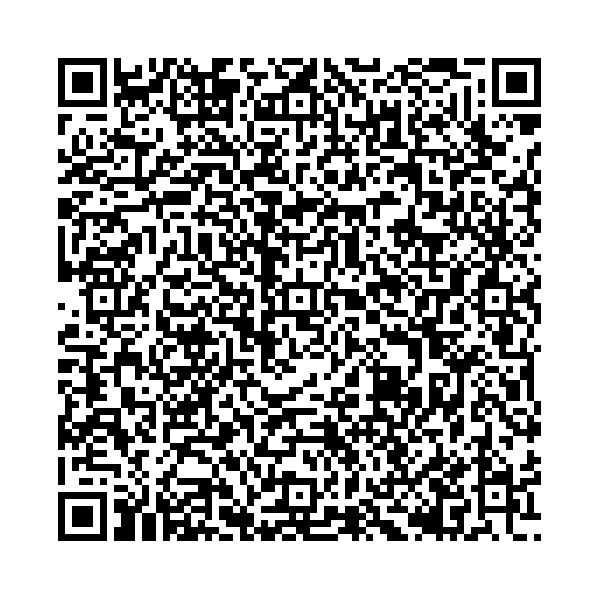
\includegraphics[width=.8\linewidth]{badqr.png}
\caption{Un code QR généré par ZXing que ZXing en soi ne peut pas décoder dans l'expérience.}
\label{fig:qr:bad-code}
\end{figure}

\subsection{Paramètres des expériences}

L'expérience vise à identifier la combinaison de paramètres qui permettraient de maximiser la bande passante et de minimiser le taux d'erreur de transmission de codes. Les paramètres qui ont été considérés sont les suivants.

\subsubsection{Résolution de codes}

Le premier paramètre est la taille de données de codes (c.-à-d. le nombre de bits de données contenues dans chaque code) et la taille physique (le nombre de pixels utilisés pour afficher le code sur l'écran). Nous avons varié la taille des données par incréments de 500 bits, de 500 à 4500 bits. Comme le montre le tableau \ref{tab:qr:sample-sizes}, le plus grand code QR, qui contient 4500 bits de données en utilisant le niveau le plus élevé de correction d'erreur, occupe 101 $\times$ 101 modules. Nous avons aussi fixé la taille physique de codes à 700 $\times$ 700 pixels sur l'écran, ce qui rend chaque module un carré d'au moins 6 $\times$ 6 pixels.

\begin{table}[ht]
\begin{center}
\begin{tabular}{llll}
Nombre de bits & Niveau de correction & Version de symbole & Taille de symbole \\
de données d'entrées & d'erreur & & \\
\hline
\multirow{2}{*}{500} & L & 3 & 29$\times$29\\
& H & 5 & 37$\times$37\\
\hline
\multirow{2}{*}{1000} & L & 5 & 37$\times$37\\
& H & 9 & 53$\times$53\\
\hline
\multirow{2}{*}{1500} & L & 6 & 41$\times$41\\
& H & 11 & 61$\times$61\\
\hline
\multirow{2}{*}{2000} & L & 8 & 49$\times$49\\
& H & 13 & 69$\times$69\\
\hline
\multirow{2}{*}{2500} & L & 9 & 53$\times$53\\
& H & 15 & 77$\times$77\\
\hline
\multirow{2}{*}{3000} & L & 10 & 57$\times$57\\
& H & 17 & 85$\times$85\\
\hline
\multirow{2}{*}{3500} & L & 11 & 61$\times$61\\
& H & 18 & 89$\times$89\\
\hline
\multirow{2}{*}{4000} & L & 12 & 65$\times$65\\
& H & 20 & 97$\times$97\\
\hline
\multirow{2}{*}{4500} & L & 13 & 69$\times$69\\
& H & 21 & 101$\times$101\\
\hline
\multirow{2}{*}{5800} & L & 19 & 93$\times$93\\
& H & 30 & 137$\times$137\\
\hline\end{tabular}
\caption[Tailles d'échantillons]{Tailles d'échantillons de codes QR, selon leurs tailles de données et les niveaux de correction d'erreurs \citep{iso18004}}
\label{tab:qr:sample-sizes}
\end{center}
\end{table}

\subsubsection{Fréquence de codes}

Le deuxième paramètre expérimental que nous avons considéré est la fréquence de codes, c'est-à-dire le nombre de codes affichés par unité de temps. Nous avons d'abord choisi 2, 4, 6, 8 et 10 codes par seconde (cps), et également considéré jusqu'à 16 cps dans une phase ultérieure de l'expérience.

\subsubsection{Niveau de correction d'erreur}

Comme nous l'avons vu, les codes QR comprennent des données supplémentaires destinées à la correction d'erreurs. Nous avons donc aussi varié le niveau de correction d'erreur dans chaque expérience, en utilisant soit son réglage le plus élevé (H) ou le plus bas (L).

\subsubsection{Résolution et fréquence de la caméra}

La résolution de la caméra n'a pas été considérée comme un paramètre expérimental. Elle était fixe à sa valeur maximale, 1920 $\times$ 1080 pixels. De même, la fréquence d'image était fixe à 30 images par seconde. Cela correspond à la vidéo à haute définition 1080p, un réglage qui devrait être trouvé dans la plupart d'appareils récents et futurs de capture vidéo. Nous avons effectué quelques tests informels avec des basses résolutions (en baisse à 640 $\times$ 480), qui étaient mondialement concluants, mais qui n'ont pas été considérés pertinents de les inclure dans notre analyse détaillée.

\subsection{Résultats des expériences}

Le produit de toutes les combinaisons de tailles de codes, de niveaux d'erreur de correction et de fréquences de codes mène à un total de 90 expériences différentes. Ces expériences ont été répétées dans les trois ensembles, qui diffèrent par la façon dont les codes ont été affichés.

\subsubsection{Affichage en une fois}

Dans la première expérience, chaque code a été affiché en séquence pour une durée de $1/f$ seconde, où $f$ est la fréquence de codes. La bande passante et le taux de décodage sont présentés dans la Figure \ref{img-exp1} pour les combinaisons de tous les paramètres.

\begin{figure}
\begin{center}
\centering
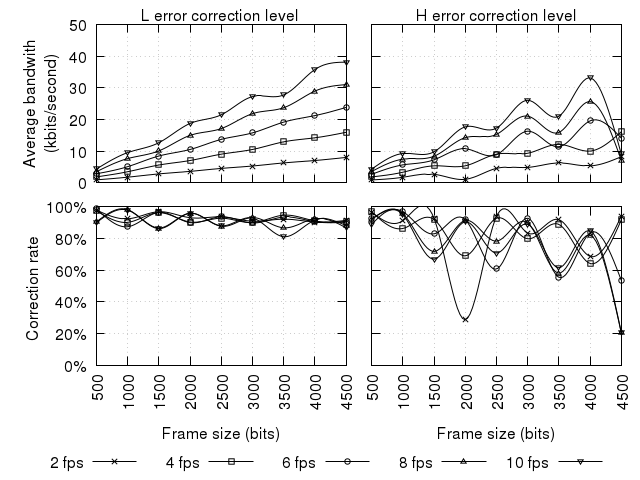
\includegraphics[width=\linewidth]{data1.png}
\caption{Bande passante et taux de décodage dans la première expérience}
\label{img-exp1}
\end{center}
\end{figure}

Comme on peut le voir, les taux de reconnaissance de niveaux plus élevé de correction étaient inférieurs à ceux de niveaux plus bas de correction, avec tous les autres paramètres étant égaux. Ceci peut être expliqué par le fait que la même quantité de données, portées dans un code avec un niveau plus élevé de correction, doit afficher plus de modules. Par exemple, selon le Tableau \ref{tab:qr:sample-sizes}, les modules d'un code 2000 bits en niveau H, sont aussi petits que ceux d'un code de 4500 bits en niveau L. Les modules plus petits, à leur tour, augmentent la difficulté de reconnaissance par la caméra. Par conséquent, une première conclusion que l'on peut tirer est que, de façon surprenante, la bande passante effective semble être améliorée en utilisant un bas niveau de correction d'erreur.

Avec les mêmes tailles de données et les mêmes niveaux de correction, la figure montre que le taux de reconnaissance diminue alors que la fréquence de codes augmente. Ceci peut être expliqué par le fait que, dans une fréquence plus élevée de codes, le même code occupe moins d'images de la caméra, et a donc moins de chances d'être correctement décodé dans l'une des images. En outre, la probabilité qu'un changement de code se produise au moment où une image soit prise (entraînant une image trouble qui montre une partie de deux différents codes) est également augmentée. En niveau L, la diminution est légère, tandis qu'en niveau H, la diminution est dramatique lorsque la taille du code atteint 3000 bits. Alors que la taille de données augmente, le taux de reconnaissance diminue constamment et considérablement.

Ces chiffres semblent indiquer que la configuration idéale pour le niveau L est 4500 bits et 10 fps, ce qui donne une bande passante effective de 39,0 kbps; pour le niveau H, 4000 bits et 10 fps mène à une bande passante de 24,6 kbps.

\subsubsection{Affichage en deux fois}

Considérant que la caméra pourrait avoir manqué plusieurs images, nous avons réalisé une seconde expérience dans laquelle chaque QR code est affiché deux fois dans une petite fenêtre du temps. Par conséquent, au lieu d'afficher chaque code une fois en $1/f$ seconde, chaque code a été entrelacé avec ses codes voisins et affiché deux fois en $1/2f$ seconde chaque fois. Ceci a pour résultat le même temps total d'exposition pour chaque code, mais augmente la diversité des images capturées par la caméra.

\begin{figure}[ht]
\begin{center}
\centering
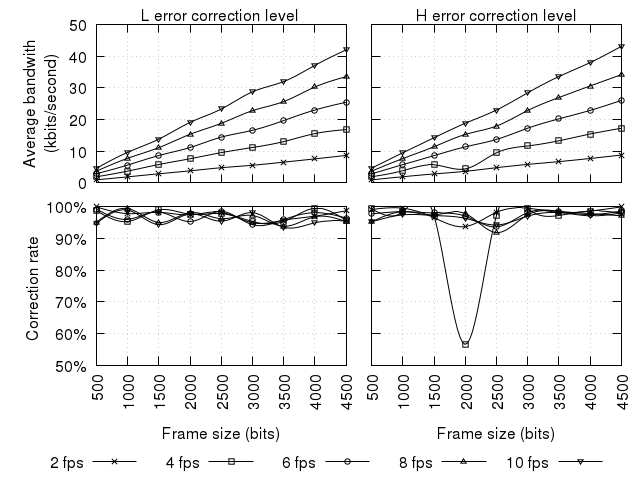
\includegraphics[width=\linewidth]{data2.png}
\caption{Bande passante et taux de décodage dans la deuxième expérience, où chaque code est affiché deux fois}
\label{img-exp2}
\end{center}
\end{figure}

Les résultats sont tracés sur la Figure \ref{img-exp2}. Ils montrent une augmentation de tous les taux de reconnaissance, qui sont maintenant tous supérieurs à 90\%. Ceci, à son tour, augmente la bande passante effective; en utilisant les mêmes paramètres que ci-dessus, on peut obtenir une bande passante de 43,0 kbps en utilisant le niveau L, et 44,1 kbps en utilisant le niveau H.

\subsubsection{Bourrage aléatoire}

Cependant, comme nous avons discuté plus tôt, les codes QR ne sont pas tous créés égaux; Avec la même résolution et le même niveau de correction d'erreur, les résultats expérimentaux indiquent que certains codes semblent être plus difficiles à reconnaître que d'autres. Par conséquent, la simple répétition de la même image en plusieurs fois n'a aucun impact sur cette intrinsèque ``dureté''. Notre troisième expérience présente encore un autre mécanisme pour augmenter le taux de reconnaissance.

Cette fois, nous avons essayé de générer les codes à partir des mêmes données d'entrée différentes en ajoutant, à la fin des données, une petite chaîne de caractères aléatoires qui est destinée à changer chaque fois où le code doit être affiché. De ce fait, les mêmes données originales, si elles sont affichées deux fois, sont préfixées à un différent bourrage aléatoire chaque fois, ce qui donne un peu différent tableau de bits. Toutefois, en vertu du schéma de codage QR, même un petit changement à la fin d'un tableau produit une forme complètement différente de points dans le code QR généré. La Figure \ref{fig:qr:difcodes} montre un exemple de ce phénomène. Par conséquent, si un code est plus difficile à reconnaître, les mêmes données sont également affichées dans une forme largement différente de points, ce qui augmente les chances d'être correctement ramassées au moins une fois.

\begin{figure}
\centering
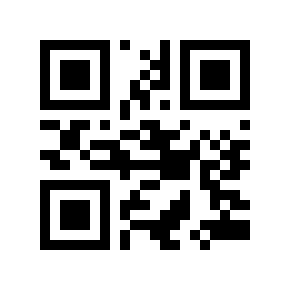
\includegraphics[width=1in]{abcdefg.jpg}~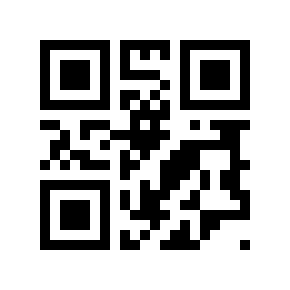
\includegraphics[width=1in]{abcdeff.jpg}
\caption{Exemples de deux codes avec les données légèrement différentes, mais avec de très différentes formes de points. Le code à gauche contient la chaîne ``abcdefg'', tandis que celui à droite contient ``abcdefg''.}
\label{fig:qr:difcodes}
\end{figure}

Bien que la raison objective que certains codes sont plus difficiles à reconnaître soit inconnue et hors sujet de ce chapitre, les résultats expérimentaux semblent confirmer cette hypothèse. Nous avons effectué une troisième expérience où chaque donnée d'entrée a été affichée trois fois avec différents codes QR générés. Le taux de reconnaissance est meilleure qu'avant lorsque la fréquence de codes est inférieure à 10 fps, comme le montre la Figure \ref{img-exp3}.

\begin{figure}[ht]
\begin{center}
\centering
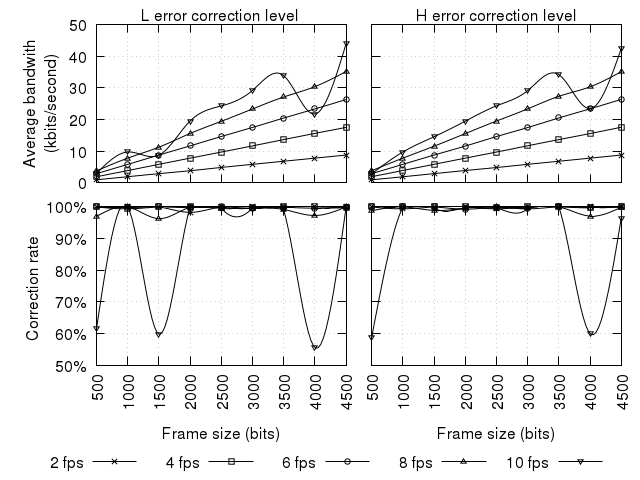
\includegraphics[width=\linewidth]{data3.png}
\caption{Troisième expérience: affichage en trois fois avec bourrage aléatoire}
\label{img-exp3}
\end{center}
\end{figure}

Ces résultats nous ont amenés à expérimenter avec les fréquences plus élevées de codes; nous avons ajouté 12 cps, 14 cps et 16 cps. Les codes ont été affichés deux fois. Comme la figure \ref{img-exp4} le montre, la bande passante maximale du résultat est 65,5 kbps en niveau L, et 68,3 kbps en niveau H, en utilisant 16 cps et les codes de 4500 bits.

\begin{figure}[ht]
\begin{center}
\centering
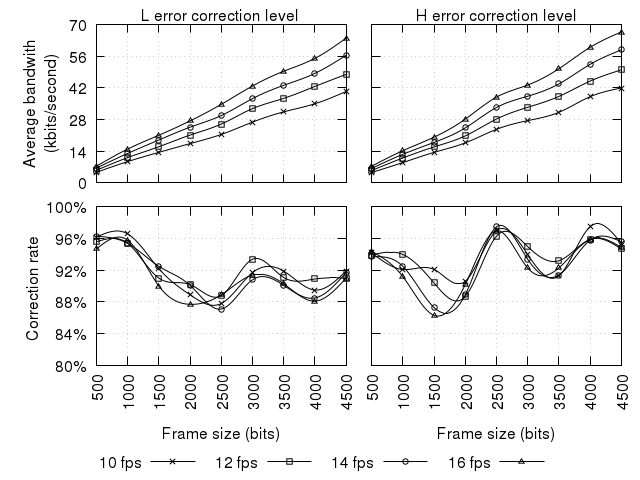
\includegraphics[width=\linewidth]{data4.png}
\caption{Quatrième expérience: affichage en deux fois et les fréquences plus élevées de codes}
\label{img-exp4}
\end{center}
\end{figure}

\subsection{Conclusions partielles}

Ces expériences initiales nous permettent de tirer quelques conclusions sur la nature d'un canal de communication de codes QR. Premièrement, bien que la fréquence plus élevée de codes et la taille plus élevée de codes aient un impact négatif sur le taux de reconnaissance, les données accrues qui peuvent être globalement portées compensent le taux plus élevé d'erreurs en termes de la bande passante effective. Deuxièmement, l'introduction de répétition et la variation de formes de points pour les mêmes données augmentent la bande passante effective; cela montre que deux codes différents pour la moitié du temps est plus efficace qu'un seul code pour le même intervalle. Troisièmement, même pour les plus petites tailles de codes, le taux d'erreur du canal est jamais zéro, ce qui indique que le canal est intrinsèquement avec perte.

A partir de ces constatations, on peut raisonnablement s'attendre qu'un flux de QR code fournisse un canal avec une bande passante effective d'environ 40 kbps, lors de l'affichage de 10 codes de 4000 bits par seconde en utilisant la technique de bourrage aléatoire et le niveau L de correction d'erreur. Le taux de décodage du canal avec ces paramètres doit être au moins 95\%. Évidement, ces constatations sont applicables à un réglage d'une caméra fixe. Elle ne prennent pas en considération la gigue potentielle, le flou ou d'autres effets qui peuvent se produire dans d'autres contextes ---bien qu'une expérience informelle décrite dans la section \ref{subsub:swipe} tende à indiquer que la technologie est relativement robuste.

%% }}} --- Section

%% -----------------------
%% Section: le protocole
%% -----------------------
\section{Un protocole de canaux de communication unidirectionnelle avec perte}\label{sec:qr:protocol} %% {{{

Dans cette section, nous proposons une approche qui utilise les codes QR continus en tant qu moyen pour réaliser une transmission unidirectionnelle de données.

\subsection{Objectifs de la conception}

Afin de mettre en \oe{}uvre un canal de communication, un protocole spécifique est essentiel; il doit être bien conçu de telle sorte que les données peuvent être sérialisées et transférées sans coût important. En outre, le protocole doit avoir la capacité de diviser les données transférées dans des images pour générer les codes QR. Le résultat est BufferTannen, un logiciel Java dédié à la sérialisation et à la transmission de données structurées sur des canaux limités de communication.\footnote{\url{https://github.com/sylvainhalle/BufferTannen}} Il fournit un ensemble de classes permettant la représentation de données structurées sous une forme binaire compacte. Contrairement à d'autres systèmes, comme Protocol Buffers de Google\footnote{\url{https://github.com/google/protobuf}}, la définition de nouveaux types de messages peuvent être effectués lors de l'exécution et ne requiert pas la compilation de nouvelles classes utilisées. De plus, les messages dans BufferTannen ne peuvent pas être codés et décodés sans connaissance préalable de leur structure. Toutefois, étant donné que les messages ne contiennent pas d'information de leur structure, ils utilisent beaucoup moins d'espace.

BufferTannen définit aussi un protocole permettant la transmission de messages. Malgré que tout canal (e.g. connexion TCP, etc.) puisse être utilisé, BufferTannen a été conçu pour l'opération sur un canal avec les spécifications suivantes, qui sont basées sur nos premiers résultats expérimentaux:

\begin{itemize}
\item Le canal est point à point. Le but est d'envoyer de l'information directement de A à B; il ne fournit pas d'adressage, de routage, etc.
\item Le canal a une bande passante faible qui est en mesure de transmettre que quelques centaines d'octets à la fois, peut-être moins de 10 fois par seconde).
\item Le canal est unidirectionnel: généralement, un côté de la communication envoie des données qui doivent être ramassées par un récepteur. Cela implique que le récepteur ne peut pas détecter la réception de données ou demander à l'expéditeur de transmettre une autre fois, comme dans des protocoles, p.ex. TCP.
\item Le canal entraîne une perte. Cependant, nous supposons que le canal fournit un mécanisme (comme une forme de somme de contrôle) pour détecter et jeter des morceaux de données corrompues.
\item Un récepteur peut commencer à écouter sur le canal à tout moment, et être capable de recevoir correctement des messages à partir de ce moment-là. Ainsi, la communication n'a pas de ``début'' formel qui pourrait être appliqué, par exemple, pour annoncer des paramètres utilisés pour l'échange.
\end{itemize}

Par conséquent, le canal de communication envisagé comme le milieu de transmission pour les messages de BufferTannen peut être similaire, à bien des égards, à un signal de diffusion lente, comme Hellschreiber \citep{hells}, télévision à balayage lente \citep{slowtv}, Télétexte \citep{teletext} ou RBDS~\citep{rbds}.

Le protocole BufferTannen vise à transmettre des messages de manière aussi fiable que possible avec ces conditions, tout en préservant l'intégrité de données et l'ordonnancement de messages. La nature de la bande passante faible du canal explique l'accent de sérialisation de messages sous une forme binaire compacte. Puisque le récepteur ne peut pas demander de aucune forme de re-transmission, le protocole doit fournir le mécanisme qui retransmet automatiquement les messages afin de maximiser leurs chances d'être ramassés, alors qu'en même temps il ne doit pas confondre une re-transmission avec un nouveau message ayant un contenu identique. En outre, parce que le récepteur peut commencer à écouter à tout moment, et que le schéma de messages doit être connu afin de les décoder, les schémas de la communication doivent également être transmis à intervalles périodiques.

\subsection{Schémas}
\setcounter{paragraph}{0}

La déclaration d'une structure de données est appelée \emph{schéma}. L'information peut être représentée sous trois formes différentes:

\begin{itemize}
\item Smallscii: Une chaîne de caractères de longueur variable. Puisque BufferTannen vise à limiter autant que possible le nombre de bits requis pour représenter de l'information, ces chaînes sont restreintes à un sous-ensemble de 63 caractères ASCII (lettres, chiffres et ponctuations). Chaque caractère dans une chaîne Smallscii occupe 6 bits, et chaque chaîne se termine avec la chaîne de 6-bit \verb+000000+.

\item Integer: Le seul type numérique disponible en BufferTannen. Lorsqu'il est déclaré, les entiers, il leur est donné une ``largeur'', c.-à-d. le nombre de bits utilisés pour encoder. La largeur peut être une valeur entre 1 et 16 bits.

\item Enum: Une liste de constantes prédéfinies de Smallscii. Une énumération est applicable pour réduire davantage la quantité d'espace occupé par un élément de données lorsque son ensemble de valeurs possibles est connu à l'avance.
\end{itemize}

Ces blocs de construction de base peuvent être utilisés pour écrire des schémas en les combinant avec l'aide de structures de données composées:

\begin{itemize}
\item List: une séquence d'éléments de longueur variable, qui doivent tous être du même type (ou schéma). Les éléments dans la liste sont accessibles par leur index, en commençant par l'index 0.
\item FixedMap: une table qui associe des chaînes à des valeurs. La structure est fixe et les chaînes de caractères exacts qui peuvent être utilisés en tant que clés doit être déclarée. Cependant, chaque clé peut être associée à une valeur de type différent.
\end{itemize}

Ces constructions peuvent être mélangées librement. Ce qui suit représente la déclaration d'un schéma de messages complexes:

\begin{verbatim}
FixedMap {
  "titre" : Smallscii,
  "prix" : Integer(5),
  "chapitres" : List [
     FixedMap {
       "nom" : Smallscii,
       "longueur" : Integer(8),
       "type" : Enum {"normal", "appendice"}
     }
  ]
}
\end{verbatim}

La structure de haut niveau pour ce message est un map (délimité par \verb+{+\dots\verb+}+). Ce map a trois clés: \verb+titre+, dont la valeur associée est une chaîne Smallscii, \verb+prix+, dont la valeur associée est un entier dans la gamme 0-32 (qui occupe 5 bits), et \verb+chapitres+, dont la valeur n'est pas un type primitif, mais est une liste en soi (délimitée par \verb+[+...\verb+]+). Chaque élément de cette liste est un map avec trois clés: une chaîne \verb+nom+, un entier \verb+longueur+, et une énumération \verb+type+ dont les valeurs possibles sont \verb+normal+ ou \verb+appendice+.

Les schémas peuvent être représentés dans une représentation binaire compacte et sans équivoque comme suit.

\paragraph{Integer} La déclaration d'un entier est encodée comme la séquence de bits suivants:
%
\begin{verbatim}
ttt wwwww ddddd s
\end{verbatim}

La séquence \verb+ttt+ représente le type d'élément, encodé sur 3 bits. Un entier contient la valeur décimale 6. La séquence de \verb+w+ indique la largeur de l'entier en bits. La largeur elle-même est encodée en 5 bits. La séquence de \verb+d+ indique la largeur de l'entier en bits, s'il est exprimé comme une valeur delta, c.-à-d. comme la différence par rapport à un entier d'un message précédent. La largeur elle-même est encodée en 5 bits. Le seul bit \verb+s+ est le signe drapeau. Si la valeur est 0, l'entier est non signé; si elle est 1, l'entier est signé. Notez que des entiers exprimés en valeurs delta sont toujours codés comme les entiers signés; par conséquent, ce drapeau s'applique uniquement aux entiers qui se produisent en tant que valeurs complètes.

\paragraph{Smallscii} La déclaration d'une chaîne Smallscii est simplement encodée comme trois bits représentant le type d'élément; une chaîne contient la valeur décimale 2.

\paragraph{Enum} Une énumération doit fournir la liste de toutes les valeurs possibles qu'elle peut prendre. Elle est formellement représentée comme suit:
%
\begin{verbatim}
ttt llll [ssssss ssssss ... 000000 ...
 ssssss ssssss ... 000000]
\end{verbatim}

Le type d'élément est la valeur décimale 1, et la séquence \verb+llll+ est le nombre d'éléments dans l'énumération, encodé sur 4 bits. Ce qui suit est une concaténation de chaînes Smallscii qui définissent les valeurs possibles de l'énumération. Chaque caractère est encodé sur 6 bits, et la fin d'une chaîne est signalée par la séquence de 6 bits \verb+000000+.

\paragraph{List} La déclaration d'une liste est la suivante:
%
\begin{verbatim}
ttt llllllll ...
\end{verbatim}

Le type d'élément est la valeur décimale 3; le 8-bit séquence \verb+llllllll+ définit le nombre maximal d'éléments dans la liste. Ce qui suit est la déclaration du type d'élément des éléments dans cette liste.

\paragraph{FixedMap} Le dernier type d'élément est le map fixe, déclaré comme suit:
%
\begin{verbatim}
ttt [ssssss ssssss ... 000000 ddd...]
\end{verbatim}

Le type d'élément est la valeur décimale 4; ce qui suit est une chaîne Smallscii qui définit le nom d'une clé, suivie par la déclaration du type d'élément pour cette clé; ceci est répété pour autant de clés que le map déclare.

\subsection{Messages}
\setcounter{paragraph}{0}

Un \emph{message} est une instance d'un schéma. Par exemple, ce qui suit est un message possible en respectant le schéma précédent:

\begin{verbatim}
{
  "titre" : "hello world",
  "prix" : 21,
  "chapitres" : [
    {
      "nom" : "chapitre 1",
      "longueur" : 3,
      "type" : "normal"
    },
    {
      "nom" : "chapitre 2",
      "longueur" : 7,
      "type" : "normal"
    },
    {
      "nom" : "conclusion",
      "longueur" : 2,
      "type" : "chapitre"
    }
  ]
}
\end{verbatim}

Le lecteur qui est familier avec JSON ou des notations similaires remarquera des fortes similitudes entre BufferTannen et ces langages. Effectivement, les éléments d'un message peuvent être interrogés en utilisant une syntaxe similaire à JavaScript. Par exemple, en supposant que \verb+m+ est un objet qui représente le message ci-dessus, la récupération de la longueur du deuxième chapitre serait écrite comme l'expression:

\begin{verbatim}
m[chapitres][1][longueur]
\end{verbatim}

Ceci amène la valeur \verb+chapitres+ de la structure de haut niveau (une liste), puis le deuxième élément de cette liste (index 1), puis la valeur \verb+longueur+ de l'élément de map correspondant.

Avec les schémas, les messages peuvent être représentés sous une forme binaire compacte.

\paragraph{Smallscii} Les chaînes sont représentées comme une séquence de caractères de 6 bits, terminée par la fin du délimiteur de chaîne \verb+000000+.

\paragraph{Integer} Les nombres sont représentés par la séquence de bits qui encode leur valeur, sans aucune séquence de terminaison: le nombre de bits à lire est dicté par la taille de l'entier, tel que spécifié par l'élément de schéma correspondant. Si l'entier est signé, le premier bit représente le signe (0 = positif, 1 = négatif) et le reste de la séquence représente la valeur absolue.

\paragraph{Enum} Une énumération est simplement fabriquée en bits de séquence correspondant à la valeur appropriée. Encore, le nombre de bits à lire est dicté par la taille de l'énumération, tel que spécifié dans le schéma du message à lire. Par exemple, si l'énumération définit 4 valeurs, alors 2 bits seront lus. La valeur numérique $i$ correspond à la $i$-ème chaîne déclarée dans l'énumération.

\paragraph{List} Une liste commençant par 8 bits enregistre le nombre d'éléments de la liste. Le reste de la liste est la concaténation de la représentation binaire de chaque élément de la liste. Puisque le type de chaque élément et le nombre de ces éléments à lire sont tous deux connus, aucun délimiteur n'est nécessaire entre chaque élément ou à la fin de la liste.

\paragraph{Fixed Map} Le contenu d'un map fixe est simplement la concaténation de la représentation binaire de valeur de chaque map. La clé auquel chaque valeur est associée, et le type de valeur à lire, sont précisés dans le schéma du message à lire, et devraient apparaître exactement dans l'ordre où ils ont été déclarés. Cela nous évite de répéter les clés de maps dans chaque message.

\subsection{Lire et écrire des messages}

En BufferTannen, les deux schémas et des instances de schémas sont représentés par le même objet, appelé \verb+SchemaElement+. Un SchemaElement vide doit d'abord être instancié en utilisant certains schémas; cela peut être effectué soit par:

\begin{itemize}
\item Lire une chaîne de caractères formatée comme ci-dessus; soit par

\item Lire une chaîne binaire qui contient un codage du schéma. En effet, en BufferTannen les messages et les schémas peuvent être transmis sous une forme binaire sur un canal de communication, et une méthode est fournie pour exporter le schéma d'un message dans une séquence de bits.
\end{itemize}

Une fois qu'un SchemaElement vide est obtenu, il peut être rempli avec des données, encore de deux façons:

\begin{itemize}
\item Lire une chaîne de caractères formatée comme ci-dessus; ou

\item Lire une chaîne binaire qui contient un codage des données.
\end{itemize}

Il y a des méthodes similaires pour fonctionner en sens inverse, et pour \emph {écrire} le schéma ou le contenu de données d'un message comme une chaîne de caractères ou une chaîne binaire. De cette façon, les messages et les schémas peuvent être librement encodés/décodés en utilisant des chaînes de textes lisibles ou des chaînes binaires compactes.

Comme on peut le voir, pour lire ou écrire un message, il faut d'abord instancier un objet avec un schéma. En fait, l'essai de décodage d'un flux de données sans publicité du schéma sous-jacent provoquera une erreur, même si le flux contient correctement des données formatées. De même, l'essai de lecture de données qui utilise un  schéma avec un objet instancié avec un autre schéma provoquera également une erreur. En d'autres termes, aucune donnée ne peut être lue ou écrite sans connaissance du schéma correct.

Cela peut sembler restrictif, mais il permet BufferTannen d'optimiser fortement la représentation binaire de messages. En l'absence d'un schéma connu, chaque message aurait besoin de porter, en plus de ses données réelles, de l'information de sa propre structure.

En pratique, grâce à lui, les répétitions de la description de son schéma dans chaque message se trouvent toutes dans les données du message. Au contraire, si le schéma est connu, toutes ces informations de signalisation peuvent être jetées: lors de la réception d'une séquence de bits, un lecteur qui possède le schéma connaît exactement le nombre de bits à lire, les données qu'il représente et la position où les données sont placées dans le structure de message. Cela implique toutefois qu'un récepteur qui ne connaît pas le schéma à appliquer n'a aucune idée sur la façon de traiter une chaîne binaire.

Pour illustrer l'intérêt de BufferTannen comme un schéma de codage de messages, nous considérons l'exemple de transmettre de événements à partir d'un jeu vidéo à un moniteur externe.

\subsection{Segments}
\setcounter{paragraph}{0}

Les messages et les schémas sont encapsulés dans une structure appelée \emph{segment}. Un segment peut être de quatre types:

\paragraph{Segments de message} contiennent la représentation binaire d'un message, avec un numéro séquentiel (utilisé pour préserver l'ordre des messages reçus), ainsi que le numéro se référant au schéma qui doit être utilisé pour décoder le message. Un segment de message est constitué d'un en-tête structuré comme suit:

\begin{verbatim}
tt nnnnnnnnnnnn wwwwwwwwwwww ssss ...
\end{verbatim}

L'en-tête commence par deux bits décrivant le type du segment; un segment de message contient la valeur décimale 1. Les sections \verb+n+ et \verb+w+ décrivent le numéro séquentiel et la longueur totale du segment, qui sont tous deux encodées sur 12 bits. Les quatre bits de \verb+s+ fournissent le numéro de schéma dans la banque de schéma qui devrait être utilisée pour lire ce segment. Le reste du segment est composé d'un map, d'une liste, d'une chaîne Smallscii ou d'un nombre, dont la représentation binaire a été décrite ci-dessus.

\paragraph{Segments de schéma} contiennent la représentation binaire d'un schéma, qui est associé à un numéro. Plusieurs schémas peuvent être utilisés dans la même communication, donc une banque de schémas identifiés par leurs numéros est crée. Un segment de schéma consiste en un en-tête structuré comme suit:

\begin{verbatim}
tt nnnnnnnnnnnn ssss ...
\end{verbatim}

L'en-tête commence par deux bits décrivant le type du segment; un segment de schéma contient la valeur décimale 2. La section \verb+n+ décrit le numéro séquentiel du segment, et la section \verb+s+ donne le numéro du schéma dans la banque de schémas auquel ce segment devrait être attribué. Le reste du segment est constitué d'une chaîne binaire décrivant le schéma, dont la représentation a été décrite ci-dessus.

\paragraph{Segments de blob} sont destinés à transporter des données binaires brutes selon le protocole BufferTannen.

\paragraph{Segments deltas} contiennent la représentation binaire d'un message exprimé comme la différence (``delta'') entre ce message et le précédent utilisé comme référence. Les segments deltas sont utilisés pour comprimer davantage la représentation d'un message, dans le cas où les messages ne changent pas beaucoup pour un intervalle de temps.

\begin{verbatim}
tt nnnnnnnnnnnn wwwwwwwwwwww rrrrrrrrrrrr...
\end{verbatim}

L'en-tête commence par deux bits décrivant le type du segment; un segment delta contient la valeur décimale 1. Les sections \verb+n+ et \verb+w+ décrivent le numéro séquentiel et la longueur totale du segment, qui sont tous deux encodées sur 12 bits. La section \verb+r+ donne le numéro séquentiel d'un autre segment, en rapport avec laquelle le delta du segment actuel est exprimé. Ce qui suit est une chaîne binaire qui décrit le contenu de la ``différence'', et il doit être calculé par rapport à ce segment pour obtenir le contenu de l'actuel.

Le calcul du delta est récursivement effectué sur chaque élément des deux messages pour comparer dans l'ordre où ils se produisent. Chaque type d'élément est défini comme suit.

\begin{itemize}
\item Smallscii strings: si les chaînes correspondantes sont identiques, émettre le seul bit \verb+0+. Sinon, émettre le bit \verb+1+ qui est suivi par la chaîne Smallscii du message cible.

\item Integers: si les numéros correspondants sont identiques, émettre le seul bit \verb+0+. Dans le cas contraire, émettre le bit \verb+1+ suivi par la différence entre la source et le nombre entier cible.

\item Enumerations: si la valeur correspondante du type énuméré est la même, émettre le seul bit \verb+0+. Autrement, émettre le bit \verb+1+ suivi par la valeur de l'entier correspondant à l'index de la valeur dans le message cible.

\item Lists: si les deux listes ont les mêmes éléments dans le même ordre, émettre le seul bit \verb+0+. Sinon, émettre le bit \verb+1+ suivi par la représentation binaire de la liste des cibles.

\item FixedMaps: appliquer récursivement les règles précédentes pour chaque clé du map.
\end{itemize}

On peut voir que les segments delta appliquent uniquement une forme grossière de comparaison. Par exemple, on ne tente pas de détecter si les deux listes diffèrent par l'addition ou la suppression d'un élément; le contenu de la liste est retransmis en intégralité chaque fois qu'il n'est pas identique à l'original. Néanmoins, cette technique permet de réaliser des économies substantielles chaque fois qu'une partie d'une structure de données reste identique d'un message à l'autre.

\subsection{Images}
\setcounter{paragraph}{0}

Le canal de communication envoie des données binaires en unités appelées \emph{images}. Une image est simplement un ensemble de segments concaténés sous une forme binaire, précédés d'un en-tête contenant le numéro de version du protocole (actuellement ``1'') et la longueur (en bits) du contenu de l'image. Formellement, la structure binaire d'une image est la suivante:

\begin{verbatim}
vvvv nnnnnnnnnnnnnn ffff... ffff...
\end{verbatim}

La section \verb+v+ est constituée du numéro de version de 4 bits du protocole, suivi de 14 bits indiquant la longueur (en bits) de l'image. Chaque segment est ajouté directement à cet en-tête de 18 bits. Parce que l'en-tête de chaque segment contient sa propre longueur, aucune autre transformation n'est nécessaire pour décoder correctement les données de segment.

Lorsque de nombreux segments sont en attente d'être transmis, le protocole tente d'adapter autant de segments que possible (dans un ordre séquentiel) au sein de la taille maximale d'une image avant de l'envoyer. Cette taille maximale peut être modifiée pour correspondre aux spécificités du canal de communication qui est utilisé. Dans l'incarnation actuelle du protocole, les segments ne peuvent pas être fragmentés en plusieurs images. Ainsi, un segment ne peut pas dépasser la taille maximale d'une image.

Chaque image est ensuite convertie en un code QR, avec son contenu binaire base64-encodé comme le texte de codes. Ce code QR peut alors être reconnu sur le site de réception, converti en une séquence binaire, et analysé et transmis aux images, aux segments et aux messages à travers l'application des transformations inverses.

\subsection{Modes de streaming}
\setcounter{paragraph}{0}

BufferTannen est conçu avec deux modes d'envoi, respectivement appelés le mode ``Lake'' et le mode ``Stream''.

Le mode Lake est destiné à l'envoi d'une pièce finie de données, comme un fichier, ou une séquence de messages BufferTannen dont le contenu complet est connu à l'avance. Les données à envoyer sont divisées en un ensemble fini de segments, et toute la séquence de segments est émise à plusieurs reprises à travers des codes QR. Si des images sont manquantes ou mal décodées, la répétition infinie de tous les segments permet d'attraper les données manquantes à la boucle suivante. Finalement, les erreurs de décodage peuvent indiquer que les données doivent être lues pour plus d'une boucle avant qu'elles soient complètement reçues.

L'utilisation du mode Lake peut être détectée par des images transportant une valeur non nulle à leur champ d'en-tête de ``segments totaux''. Ainsi, un récepteur qui commence à lire à tout moment la séquence d'images sait combien de segments doivent au total être reçus, et la position relative de chaque segment dans les données pour être reconstruite. Cela rend le mode Lake un schéma de transmission optique de données relativement lente, mais très robuste.

En mode Stream, les données sont constamment lues en segments qui forment alors un flux d'images, et les images sont immédiatement envoyées. Le processus de lecture arrête seulement quand il n'y a plus de données à lire. Les images déjà envoyées sont supprimées de la mémoire, donc il n'y a aucun moyen de renvoyer les données à plusieurs reprises. Cependant, pour le bien de la cohérence des données, nous avons fait un tampon pour les clones des images envoyées, et après avoir envoyé une quantité spécifique d'images récupérées à partir des données originales, les images dans la mémoire tampon sont renvoyées à nouveau, puis enlevées de la mémoire tampon . Par conséquent, le mode Stream est destiné à envoyer des données en temps réel, généralement là où la perte de données est acceptable et la consistance peut être légèrement sacrifiée (par exemple audio ou vidéo).

\begin{figure*}
\centering
\begin{verbatim}
--------------------------------------------------------------------------
Sending mode:        lake
Buffer state:        [||>       ||:.::||:|||] 59% (130/219)
Progress:            0408/0000 (13.8 sec @30 fps)
Link quality:        22/30 [*******   ] (73%)  Global:   339/454 (74%)
Data stream index:   0
Resource ident.:     myfile.jpg
Processing rate:     35 ms/frame (27 fps)
--------------------------------------------------------------------------
\end{verbatim}
\caption{Une partie de l'interface texte du récepteur de codes QR qui fonctionne en mode Lake}
\label{fig:qr:lake-gui}
\end{figure*}

La Figure \ref{fig:qr:lake-gui} montre une partie de l'interface texte de notre mise en œuvre de récepteur de codes QR. L'interface montre que les images étant reçues sont en mode Lake. Le champ d'état de tampon indique la progression de la réception. Dans cet exemple, il montre que les segments 130 sur 219 ont été correctement reçus; la barre de texte à gauche indique à quelles parties de la séquence totale ces segments correspondent. Une section de la séquence qui n'a pas été reçue du tout est indiquée par un espace vide; les parties de plus en plus complètes de la séquence sont représentées respectivement par les symboles \verb+.+, \verb+:+ et \verb+|+. Le symbole \verb+>+ indique la position relative du dernier segment qui a été lu correctement.

Le champ ``Link quality" donne une indication en temps réel du taux de décodage. Il montre que 22 des 30 dernières images capturées par la caméra ont été correctement décodées, et que globalement, 339 images ont été décodées sur 454 images capturées. L'identifiant de ressource et l'index de flux de données, portés par chaque image, sont également affichés.

\subsection{Résultats expérimentaux}
\setcounter{paragraph}{0}

Les expériences de la section \ref{sec:qr:experiments} ont confirmé notre intuition que les flux de codes optiques sont un canal de communication intrinsèquement peu fiable et à faible bande passante. La compacité du protocole BufferTannen peut être motivée par un exemple de la vérification de l'exécution. Un jeu vidéo particulier, appelé Pingus, a été instrumenté pour produire des événements qui contiennent l'état de chaque personnage dans le jeu. Le schéma de ces événements est illustré à la figure \ref{fig:qr:pingus-schema}.

\subsubsection{Transfert de fichiers}

\begin{figure}
\centering
\begin{verbatim}
FixedMap {
  "pingus" : List [
    FixedMap [
      "id" : Integer(6),
      "x" : Integer(10),
      "y" : Integer(10),
      "velocity-x" : Integer(4),
      "velocity-y" : Integer(4),
      "state" : Enum {"floater",
         "basher", "builder",
         "athlete", "normal"}
    ]
  ]
}
\end{verbatim}
\caption{Le schéma d'événements produits par un jeu vidéo instrumenté.}
\label{fig:qr:pingus-schema}
\end{figure}

Un événement contient généralement des données pour 50 caractères, ainsi la structure map est répétée autant de fois. L'envoi d'un tel événement en format texte clair, sans aucun espace, prend environ 3750 octets. À un fréquence de 30 événements par seconde, il prend 879 kbps de bande passante pour transmettre le flux d'événements. Le même événement dans BufferTannen prend 1.856 bits, ou 232 octets. Cela divise par plus de 16 les exigences de bande passante pour envoyer un flux de ces événements, ce qui donne une bande passante de 54 kbps.\footnote{Envoi de la même chaîne de caractères en Gzip se rétrécit vers à 716 octets, ce qui rend la compression standard une alternative moins attrayante dans ce contexte.} Dès cet instant, les segments de delta peuvent être utilisés pour réduire davantage la bande passante du flux, et transmettre les événements restants en utilisant un peu plus de 100 octets chacun, qui consomme une bande passante d'environ 24 kbps. Nos expériences précédentes montrent que cela est dans la gamme de ce que l'on peut raisonnablement s'attendre à transmettre à travers les codes QR.

Nous avons ensuite testé la capacité du protocole BufferTannen pour atténuer ces défauts, à travers son utilisation de répétition et sa représentation binaire compacte \footnote{Une vidéo de BufferTannen en action est disponible en ligne: \url{https://www.youtube.com/watch?v=GSL0md0TlY8}}

Nous avons choisi d'encoder des données en codes de 4000 bits, qui, après l'encapsulation de BufferTannen, équivaut à un code QR d'environ 5800 bits. Avec la combinaison de 5800 bits et du niveau L de correction, selon le Tableau \ref{tab:qr:sample-sizes}, la taille de symboles est d'environ 93 $\times$ 93 qui est entre les combinaisons de 3500 bits, du niveau H et de 4000 bits, du niveau H. D'après le résultat de la dernière expérience, les combinaisons de 4000 bits, du niveau H et tous les fps ont un taux de plus 95\% de correction   qui est fiable. D'autre part, les fréquences de codage sont 4, 6, 8, 10, 12 images par seconde. Selon la dernière expérience, cette configuration est fiable et censée être capable de fournir, respectivement 23.2--69.6 kbps et 16.0--48.0 kbps de bande passante. Étant donné l'application pratique, nous avons choisi de transférer un fichier d'exemple dont la taille est de 37,656 octets, et nous avons effectué chaque expérience 20 fois.

Le résultat de l'expérience du mode Lake dans la Figure \ref{img-explake} montre que la meilleure valeur de fps est de 10, et dans ce cas, le fichier d'exemple avait besoin d'être transféré en moyenne 2,4 fois pour s'assurer que le récepteur pourra obtenir toutes les images. Le temps passé en moyenne est de 17,27 secondes, et la bande passante est donc environ 17,0 kbps.

\begin{figure}[ht]
\begin{center}
\centering
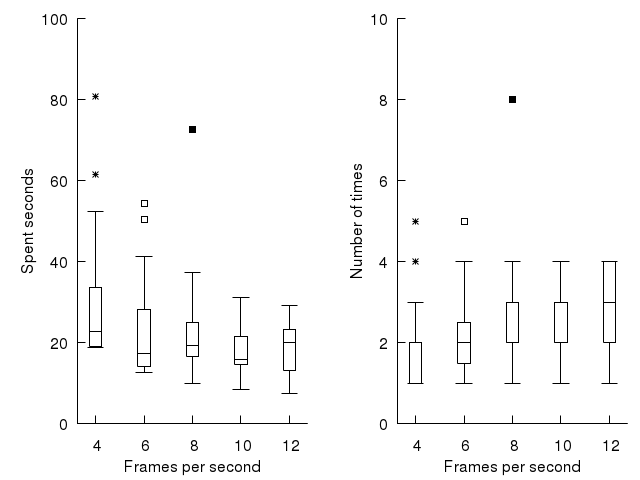
\includegraphics[width=\linewidth]{lake.png}
\caption{Temps de l'envoi des données en mode Lake}
\label{img-explake}
\end{center}
\end{figure}

En mode Stream, le pourcentage de codes reçus est important. Dans l'expérience, selon la Figure \ref{img-expstream}, les taux moyens d'achèvement de toutes les configurations sont plus de 99\%, et la configuration de 12 fps a besoin d'environ 13,11 secondes pour envoyer toutes les images avec un canal de streaming de données de 22,4 kbps .

\begin{figure}[ht]
\begin{center}
\centering
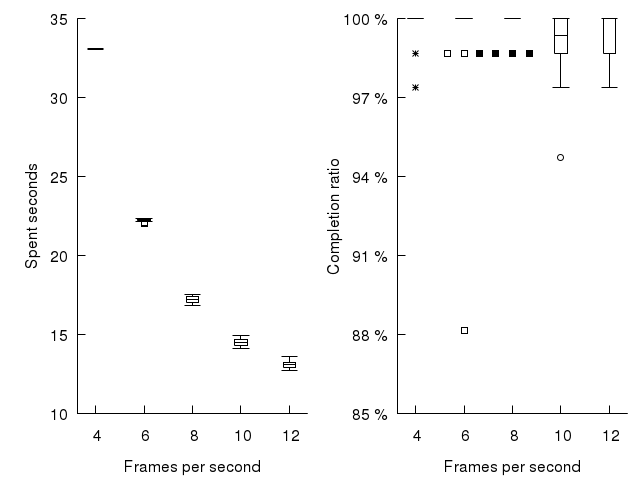
\includegraphics[width=\linewidth]{stream.png}
\caption{Temps de l'envoi des données en mode Lake Stream}
\label{img-expstream}
\end{center}
\end{figure}

\subsubsection{Glisser du papier}\label{subsub:swipe}

La capacité d'envoi des flux de données en mode Lake peut également être utilisée pour compléter la capacité intrinsèquement limitée de codes QR. Lors de l'affichage d'un code imprimé sur une feuille de papier, de grandes quantités de données peuvent être seulement apportées par l'augmentation de la résolution de codes; cependant, la résolution ne peut être augmentée jusqu'à une limite certaine et prédéfinie.\footnote{4296 caractères alphanumériques ou 3222 octets en codage Base-64.} En outre, pour des résolutions plus élevées, le code peut devenir difficile à reconnaître en utilisant des caméras en niveau d'entrée et en basse résolution. Par conséquent, c'est prudent de supposer que, avec l'aide de la technologie existante de codes QR, un maximum de  3000 octets de données peuvent être transférées à travers un code QR.

Cette limitation peut être surmontée par l'utilisation du protocole BufferTannen. Bien qu'aucun code dont la taille est supérieure à environ 4000 octets ne puisse être créé, plusieurs de ces codes peuvent être alignés sur un morceau de papier. Chacun de ces codes peut être formaté pour contenir une image unique de données envoyées par le protocole BufferTannen en mode Lake. Il suffit à l'utilisateur de glisser la caméra sur ces codes; en vertu du mode Lake, l'ordre dans lequel les codes sont scannés n'est pas pertinent, et les pièces complètes de données peuvent être correctement reconstruites à partir des images individuelles. c'est donc possible de théoriquement transmettre des quantités illimitées de données, tout en utilisant des codes d'une résolution inférieure (cette résolution inférieure étant compensée par la présence de plus d'un code).

Pour vérifier cette affirmation, nous avons imprimé sur une feuille de papier le contenu d'un fichier de 37 ko en tant qu'une séquence de codes QR, traités comme des images par BufferTannen en mode Lake. Nous avons ensuite passé la caméra au-dessus de cette feuille de papier à une distance d'une longueur de bras (montré dans la Figure \ref{fig:qr:paper-swipe}). L'interface utilisateur du logiciel affiche en temps réel le nombre d'images restantes à décoder et leurs positions dans le flux complet, qui donne à l'utilisateur des indications de codes que passe la caméra. Il convient de noter que la caméra fonctionnait en mode ``film'', et non en mode ``snapshot''. En d'autres termes, les images ont été capturées continuellement par la caméra lorsque elle était déplacée au-dessus de la feuille; l'utilisateur n'a pas besoin de pointer et de cliquer sur chaque code QR individuel (ce qui serait fastidieux).

\begin{figure}
\centering
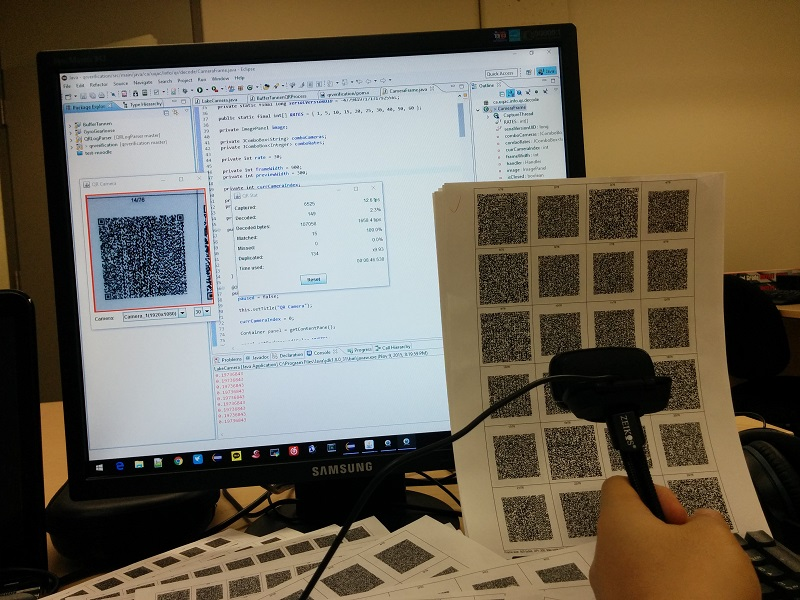
\includegraphics[width=\linewidth]{swipe.jpg}
\caption{Passer la caméra au-dessus d'un ensemble de codes QR pour reconstituer le contenu d'un fichier plus grand.}
\label{fig:qr:paper-swipe}
\end{figure}

Le niveau de correction d'erreur choisi était L et les tailles de données brutes par code que nous avons testées étaient 500, 750, 1000, 1250, 1500, 1750, et 2000 octets. Avec 500 octets, il y avait 76 codes tandis qu'avec 2000 octets, il y en avait seulement 19. Après avoir été encapsulées par le protocole BufferTannen, les tailles finales de données utilisées pour générer les codes QR sont devenues en conséquence 723, 1055, 1391, 1724, 2054, 2389 et 2722 octets. Les codes ont été imprimés à 300 ppp (points par pouces) et 600 ppp sur des papiers de bureau , et nous avons programmés pour donner 500 points à chaque bord de tous les codes dans le papier.

À 300 ppp, les codes dont la taille était de 500 à 1250 octets étaient tous décodés avec succès et en douceur. Cependant, quand la taille a atteint 1500 octets, le décodage est devenu plus problématique. Pour certains codes, nous avons dû recommencer plusieurs fois et coller la caméra près du papier pendant quelques secondes, mais parmi le total de 31 codes, trois restaient impossible à décoder. Dans le cas des codes de 1.750 et de 2.000 octets, aucun des codes n'aurait pu être décodé. Ceci peut être expliqué par le fait que les codes de densité plus élevée ont pour effet que chaque module de code est plus petit et ainsi plus difficile à capturer. Par exemple, le bord d'un code de 500-octets et du niveau L est d'environ 77 modules, de sorte que chaque module peut avoir environ 6 points dans le papier, tandis que le bord d'un code de 2000-octets et du niveau L est 149 modules, donc chaque module ne peut avoir que 3 points pour imprimer.

À 600 ppp, aucun des codes ne pourrait pu être décodé, peu importe le nombre d'octets qu'ils ont apporté. La raison en est que les codes imprimés à 600 ppp sont trop petits et la caméra doit approcher de très près au papier, mais les images capturées étaient toutes troubles et hors de foyer. Ceci semble donc que les codes imprimés à 600 ppp sont au-delà de la capacité d'une standard caméra web.

Néanmoins, cette expérience démontre la viabilité du concept de passer une caméra à travers un tableau de codes QR. Nos découvertes empiriques indiquent qu'un flux de données peut être divisé en un ensemble de codes QR d'environ 1000 octets chacun, dont le contenu correspond à des images individuelles du protocole BufferTannen qui contiennent les données de transmission. Il suffit de passer la caméra au-dessus de cet ensemble de codes, dans aucun ordre particulier, pour reconstruire le contenu complet de données du côté de l'appareil.

%% }}} --- Section

%% -----------------------
%% Section: Conclusion
%% -----------------------
\section{Conclusion}\label{sec:qr:conclusion} %% {{{

Dans ce chapitre, nous avons présenté une solution d'un canal de communication unidirectionnelle sur la base de codes QR, et réalisé des expériences pour mesurer sa performance. Nous avons d'abord testé expérimentalement les caractéristiques d'un flux de données de codes QR sous diverses conditions, et extrait les paramètres qui  maximisent la bande passante effective du canal. Toutefois, étant donné que le canal est intrinsèquement enclin à erreur et à faible bande passante, nous avons ensuite introduit BufferTannen, un protocole conçu spécialement pour ce type de canal. BufferTannen prend soin du fractionnement, de la transformation, et dans une certaine mesure avec la compression des données de transmission afin de maximiser l'efficacité du flux de codes QR. La faisabilité de cette approche a ensuite été empiriquement observée lors d'une nouvelle série d'expériences.

Même avec les limites du protocole et du canal de communication, les résultats présentés peuvent être utilisés à bon escient dans une variété de situations. Dans les environnements limités où l'utilisation du signal de radio ou de câbles est interdite ou difficile, notre approche peut fournir un moyen facile pour communiquer entre pairs, soit comme sauvegarde d'urgence ou comme moyen principal. Par ailleurs, en raison de l'évolution de la qualité des deux dispositifs d'affichage et de capture d'images, c'est possible de prévoir des vitesses de transmission accrues dans l'avenir.

Enfin, les techniques susmentionnées pourraient être transformées en une liaison de communication bidirectionnelle dans le cas de terminaux équipés d'une caméra et d'un écran. Dans un tel cas, les reconnaissances d'images correctement décodées pourraient être échangées, ce qui permettrait de renvoyer des données sur demande et d'augmenter la bande passante effective.

%% }}} --- Section